In order to test the validity of using neural networks sampled
from molecular dynamics trajectories to generate new trajectories
we train neural networks on systems of copper and silicon atoms
using the Effective Medium Theory and Stillinger-Weber potentials
respectively. These potentials have efficient implementations
through ASE and their ASAP interface, which makes
it ideal for our purposes. Additionally these potentials
have an intermediate complexity, with Stillinger-Weber explicitly
including threebody interactions, which makes them ideal
for testing whether the Behler-Parrinello method can replicate this.
At temperatures which are not too large these potentials describe
atoms in a crystalline structure in equilibrium,
and we test whether the neural network can reproduce the correct potential
energy, forces, radial distribution and mean squared displacement.
In table \ref{tab:hyperparam} we have listed the parameters we have
used in the training process. While we have used a large amount
of training images for the energy training, since this is relatively
inexpensive, 20000 training images was not a noticeable over approximately
1000-10000 images, and only seemed to affect the speed of convergence.
We finally used 1000 images to refine the force accuracy,
as we discussed in the previous chapter.
In table \ref{tab:hyperparam-test} we have listed the parameters
used for testing the neural network. For sampling data we used a larger
timestep and sampling interval
than for applying the neural network, in order to obtain
a larger diversity of configurations, though this did not appear to
matter much in the final analysis.

% Mention loss vs RMSE here...?

\begin{table}[H]
\centering
\begin{tabular}{|c c|}
\hline
Hyperparameter & Value \\
\hline \hline
    Hidden layers & $(10)$ \\
Activation & Hyperbolic tangent \\
    Time (fs) & $2 \cdot 10^6$ \\
    Timestep (fs) & 5 \\
    Sampling intervall (timesteps) & 100 \\
Max epochs & 4000 \\
Optimizer & BFGS \\
Energy coefficient & 1.0 \\
Force coefficient & 0.1 \\
\hline
\end{tabular}
\caption{Hyperparameters used in fitting.}
\label{tab:hyperparam}
\end{table}

\begin{table}[H]
\centering
\begin{tabular}{|c c|}
\hline
Hyperparameter & Value \\
\hline \hline
    Hidden layers & $(10, 10)$ \\
Activation & Hyperbolic tangent \\
    Time (fs) & $5 \cdot 10^3$ \\
    Timestep (fs) & 1 \\
    Sampling intervall (timesteps) & 10 \\
\hline
\end{tabular}
\caption{Hyperparameters used in testing.}
\label{tab:hyperparam-test}
\end{table}

\subsection{Effective Medium Theory}
The Effective Medium Theory (EMT) potential gives a good description
of the late transition metals in a Face-Centered Cubic (FCC) crystal
lattice, and has a very efficient implementation in ASE,
which makes it ideal for producing large amounts of data.
We will train on a rather small system of $4 \times 2^3 = 32$ atoms
with a temperature of 500 Kelvin since this means a larger amount of labels available
for atoms when we are only using the potential energy.
We train with only the energy for $2 \cdot 10^6$ steps
with a timestep of $\Delta t = 5.0$ fs
writing to file every 100 steps and then subsequently
train using both energy and forces for $1 \cdot 10^5$ steps
for a total of 20 000 and 1000 configurations. We train on both sets of images
for 4000 steps, where the BFGS optimizer has generally converged.
The cutoff radius is set to 5 Angstrom, using 8 radial and
16 angular functions of the G4 type.
After the calculator is trained we compare the performance
of the neural network with the EMT potential on a system
of 32 atoms with a temperature of 300 Kelvin for 5000 steps
writing to file every 100 steps.

\begin{figure}[H]
\begin{adjustbox}{max width=1.2\linewidth,center}
\centering
  \begin{subfigure}[b]{0.55\textwidth}
      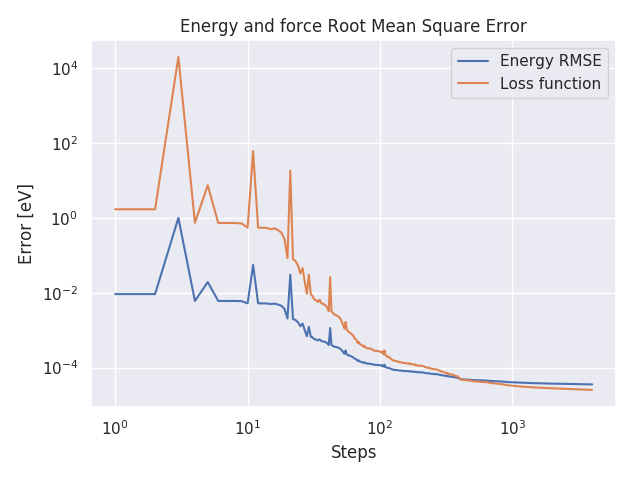
\includegraphics[width=\textwidth]{copper_energy_log.png}
      \caption{Training loss and energy RMSE.}
  \end{subfigure}
  \hfill
  \begin{subfigure}[b]{0.55\textwidth}
      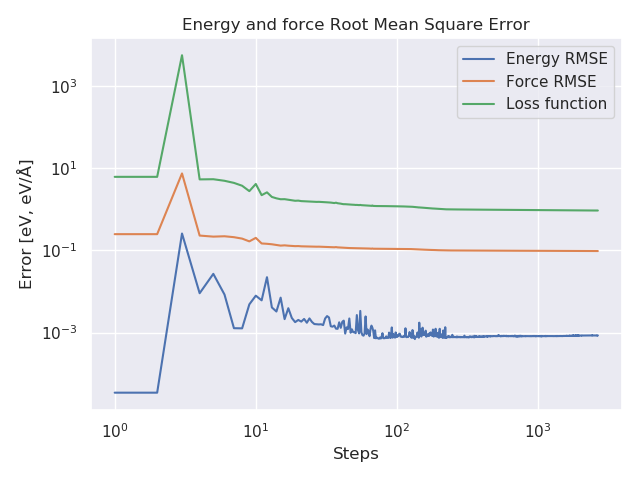
\includegraphics[width=\textwidth]{copper_force_log.png}
      \caption{Training loss and energy and force RMSE.}
  \end{subfigure}
\end{adjustbox}
\caption{Training loss, energy and force RMSE for the copper
    system (using logarithmic axes).}
    \label{fig:copper-log}
\end{figure}

In figure \ref{fig:copper-log} we have plotted the loss and root mean
squared errors for the training process.
After a few large oscillations in the beginning
the losses generally settle down and begin to decrease
more smoothly.
After approximately 500-1000 steps the network seems to have
converged, and the change in loss is much smaller than before.
Subsequently we train with forces and we observe a large increase
in the energy RMSE in exchange for a modest decrease in force RMSE,
as discussed in the previous chapter.
After training for a while both errors settle down
and converge.

\begin{figure}[H]
\begin{adjustbox}{max width=1.2\linewidth,center}
\centering
  \begin{subfigure}[b]{0.55\textwidth}
      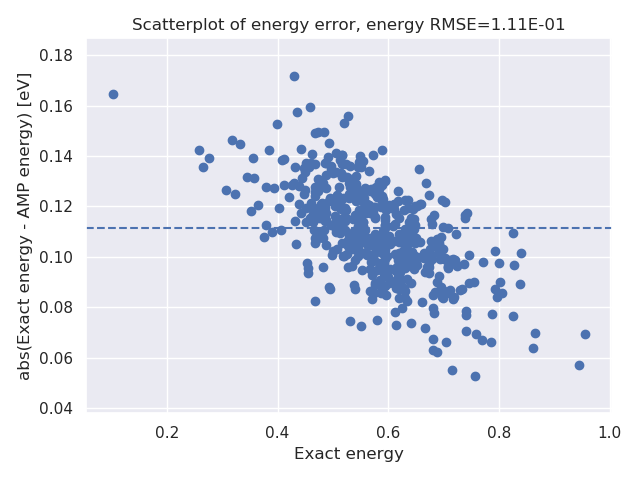
\includegraphics[width=\textwidth]{copper_energy_error.png}
      \caption{Energy error.}
    \label{fig:f1}
  \end{subfigure}
  \hfill
  \begin{subfigure}[b]{0.55\textwidth}
      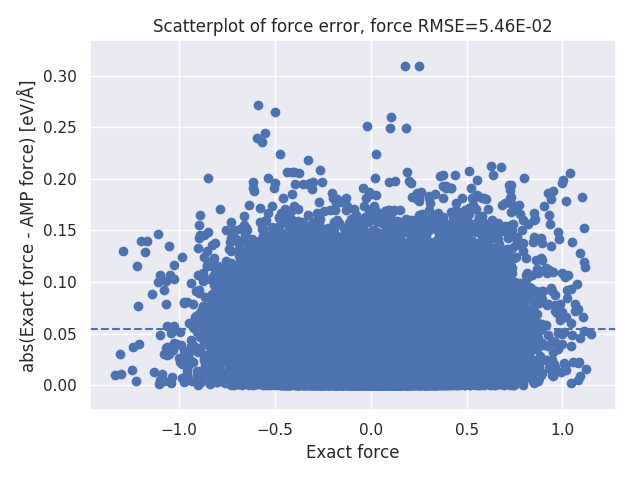
\includegraphics[width=\textwidth]{copper_force_error.png}
      \caption{Force component error.}
    \label{fig:f2}
  \end{subfigure}
\end{adjustbox}
    \caption{Energy and force component errors on test trajectory.}
    \label{fig:copper_error}
\end{figure}

In figure \ref{fig:copper_error} we have plotted the energy and force component
(i.e. in the x,y,z direction)
absolute errors on the EMT test trajectory. We obtain an energy error
of approximately 0.1 eV, with a max value of approximately 0.16 eV.
For the force errors we obtain an force RMSE of 0.05 eV/Å,
but some of the force errors considerably higher, up to
and including values of 0.3 eV/Å, which may pose
a problem for the long term stability of the system.

\begin{figure}[H]
    \centering
    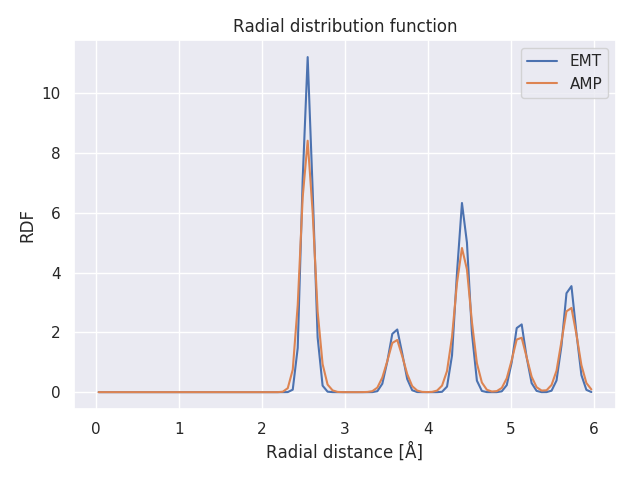
\includegraphics[width=\textwidth]{copper_rdf.png}
    \caption{AMP radial distribution function plotted against
        EMT radial distribution.}
    \label{fig:copper-rdf}
\end{figure}

In figure \ref{fig:copper-rdf} we have plotted the AMP neural network
radial distribution function compared to the EMT radial distribution.
We see that the AMP potential can reproduce the copper crystal
structure fairly well, though with smaller peaks.
As we will soon discuss, the neural network appears
to be able to reproduce the equilibrium crystal structure,
though increases in kinetic energy and translational momentum over time
makes the atoms more dispersed.

\begin{figure}[H]
    \centering
    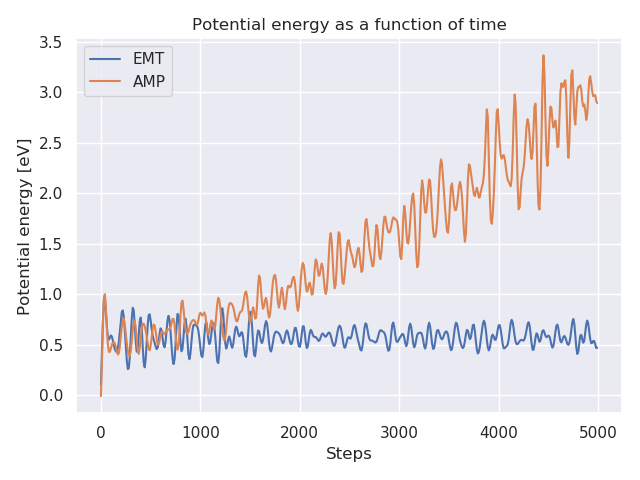
\includegraphics[width=\textwidth]{copper_pot.png}
    \caption{AMP and EMT potential energy as a function of time.}
    \label{fig:copper-pot}
\end{figure}

If we examine the potential energy as a function of time
in figure \ref{fig:copper-pot} we see that the neural network
follows the EMT potential energy fairly well for approximately
1500 steps, but then starts to significantly increase.
As the atoms are moved away from the potential
energy minimum the potential energy also starts to increase.
This most noticeable in figure \ref{fig:copper-energy},
where we have plotted the total energy as a function of time.
While the EMT energy is flat or oscillating around a mean value,
the neural network potential exhibits increasing energy over time.
At the beginning the increase in energy appears to be attributable
to an increase in kinetic energy, which may be caused by errors
in the interpolated forces from the neural network.
This increase in kinetic energy also appears to lead to an increase
in translational momentum.

\begin{figure}[H]
    \centering
    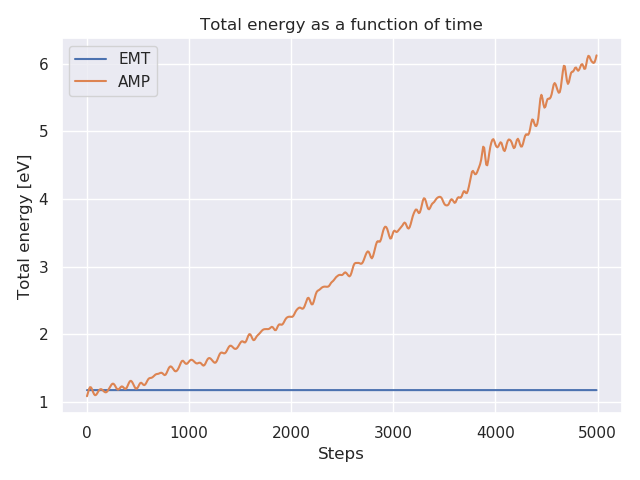
\includegraphics[width=\textwidth]{copper_energy.png}
    \caption{AMP and EMT total energy as a function of time.}
    \label{fig:copper-energy}
\end{figure}

\begin{figure}[H]
    \centering
    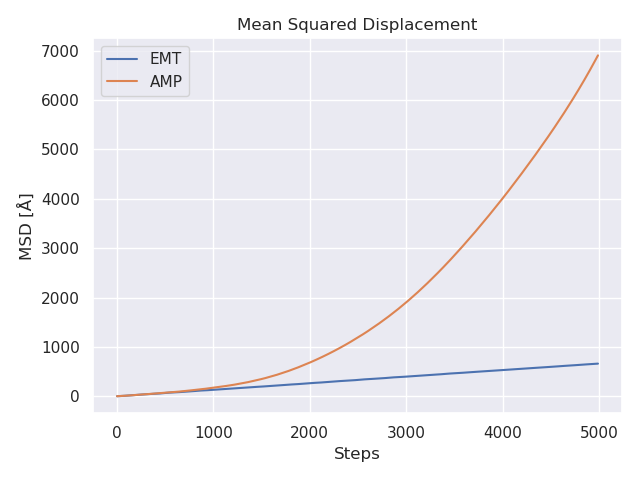
\includegraphics[width=\textwidth]{copper_msd.png}
    \caption{AMP and EMT mean squared displacements as a function of time.}
    \label{fig:copper-msd}
\end{figure}

In figure \ref{fig:copper-msd} we have plotted the mean squared
displacement, which measures mean distance travelled averaged over all
atoms in the system.
We observe that the MSD for the neural network is significantly larger
than for the EMT potential. In equilibrium we expect for a crystal lattice
that the mean squared displacement be linear, as the atoms
mostly oscillate in stable energy minimums.
For the neural network potential the motion in the system appears
to be accelerating, as the kinetic and total energy is increased
over time.

\begin{figure}[H]
\begin{adjustbox}{max width=1.2\linewidth,center}
\centering
  \begin{subfigure}[b]{0.55\textwidth}
      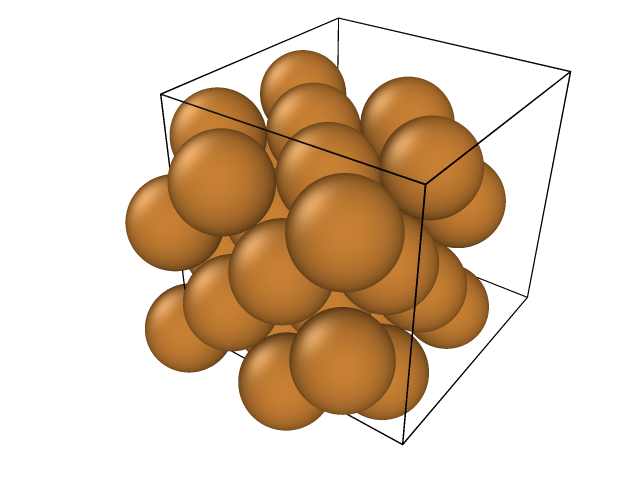
\includegraphics[width=\textwidth]{copper_t0.png}
      \caption{Copper atoms after 10 steps.}
    \label{fig:f1}
  \end{subfigure}
  \hfill
  \begin{subfigure}[b]{0.55\textwidth}
      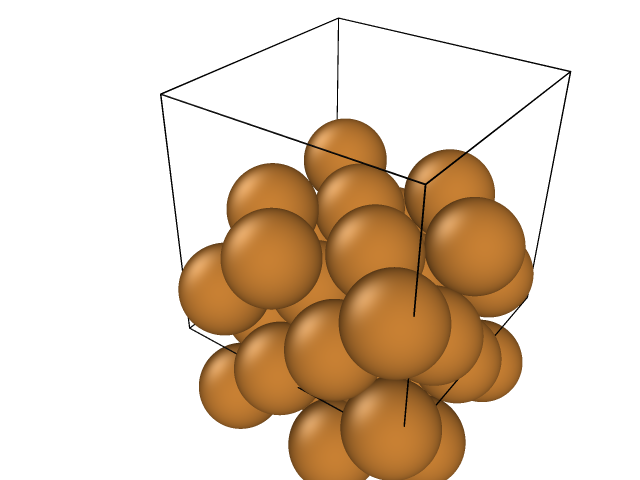
\includegraphics[width=\textwidth]{copper_tn.png}
      \caption{Copper atoms after 5000 steps.}
    \label{fig:f2}
  \end{subfigure}
\end{adjustbox}
    \caption{The system of copper atoms after 10 and 5000 timesteps.}
    \label{fig:copper_sw}
\end{figure}

If we examine the system trajectory in a program such as Ovito
\footnote{\href{https://www.ovito.org/}{Open VIsualization TOol (OVITO)}}
we find that the crystal structure has mostly remained intact, while the
system has picked up a certain amount of translational momentum.
In figure \ref{fig:copper_sw} we see that the system has moved as a whole,
although this is easier to see if you open up the trajectory file in Ovito
yourself.
This is in contrast to the EMT potential, in which the atoms vibrate in place
at this temperature, and the system remains more or less in place.
Altogether, this suggests that while the neural network potential
is able to reproduce the crystal structure, numerical errors propagate
to a linear increase in energy over time, which threatens the long-term numerical
stability of the trajectory. In order to obtain better results we would likely
require datasets containing more unlikely configurations and forces
(i.e. slightly out of equilibrium). We also generally find that the performance
improves as you add more symmetry functions, particularly radial functions
would improve the accuracy with this potential, as they are not explicitly
contained in the EMT potential. However, more symmetry functions
add significant CPU-time cost, and the set of symmetry functions would have to be pruned
to remove significant correlations.
\par
Finally, we tested the time-scaling of the neural network as the number of atoms
increased. To test this we simply made a forces call on lattices of different
sizes, which returns the force on every atom in the system.
Ideally we would have taken averages over multiple force calls, however
at this time scale we did not think it would significantly impact the results.

\begin{figure}
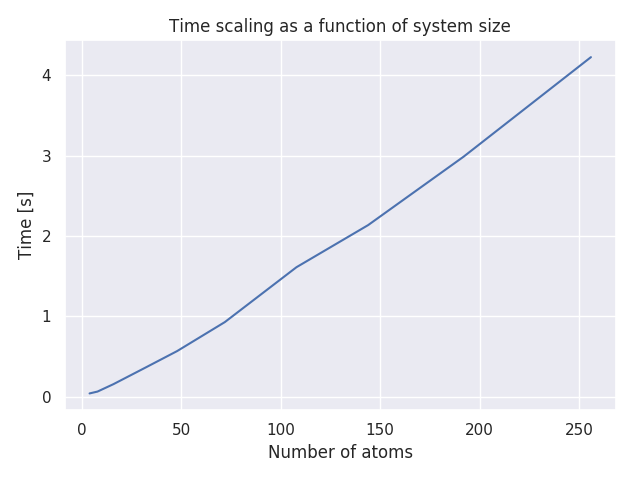
\includegraphics[width=\textwidth]{copper_scaling.png}
\caption{Time scaling of the neural network as the number of atoms increases.}
\label{fig:copper-scaling}
\end{figure}

In figure \ref{fig:copper-scaling} we see as expected that the trained neural network
scales linearly with the number of atoms, though with a significant pre-factor.
We see that it takes approximately 1 second to evaluate all the forces
for a system of 60 atoms, while it takes 4 seconds for a system of 250 atoms.
This pre-factor is dependent on the average number of neighbors
of each atom, which is again dependent on the cutoff radius.
Since the neural network has been trained with a set cutoff radius,
this radius should be considered a part of the neural network architecture
and cannot be significantly changed without impacting accuracy.
This pre-factor is of course also dependent on the time it takes to evaluate
the symmetry functions and derivatives, which is dependent on the number
and type of symmetry functions, as the angular function derivatives are significantly
more expensive to evaluate than the radial angular functions.
For the system of 250 atoms the 5000 steps take approximately 6 hours
to integrate over, which could be competitive with ab-initio methods,
though not with other classical potentials.
However, this is only on a single core, and parallelizing using neighbor list algorithms
such as thouse found in the LAMMPS package could be a big improvement without too much overhead.
While this would help deployment, training would still be too slow.
As it stands now, the symmetry function derivatives have significant parts
implemented in Python which could with some effort be moved entirely to Fortran,
such as if-tests, dictionaries and neighbor lists.
If these parts of the codebase were moved fully to a lower-level compiled
language, this would help both training and deployment, and would enable
training and testing of larger and more complex systems.

\subsection{Stillinger-Weber}
The Stillinger-Weber is a potential which describes accurately
Silicon atoms in the diamond lattice structure, and was
one of the first potentials used to describe a realistic atomic-scale
model of Silicon. It is also one of the most common examples
of a potential with a threebody interaction, and its intermediate complexity
makes it ideal for verification with for example quantum calculations
or in our case machine learning methods.
We initialize a system of 8 unit cells with 8 atoms in each unit cell
for a total of $8 \times 2^3 = 64$ atoms with velocities corresponding
to a temperature of 500 Kelvin.
As in the previous section we integrate the system over $2 \cdot 10^6$
steps using a timestep of $\Delta t = 5.0$ fs (suitable for most metals
in a crystalline structure) writing to file every 100 steps
for a total of 20 000 images for energy learning
and 1000 images used to train forces.
The neural network is trained for 4000 steps after using simulated annealing
for 2000 steps in order to search for optimal initial weights.
We then generate test sets using the Stillinger-Weber and trained neural network
for 5000 steps and compare the results using the potential energy,
radial distribution function, mean squared displacement and more.
The cutoff radius is set to $R_c = 5$ Angstrom using 14 radial and
22 angular symmetry functions of the G2 and G4 types.

\begin{figure}[H]
\begin{adjustbox}{max width=1.2\linewidth,center}
\centering
  \begin{subfigure}[b]{0.55\textwidth}
      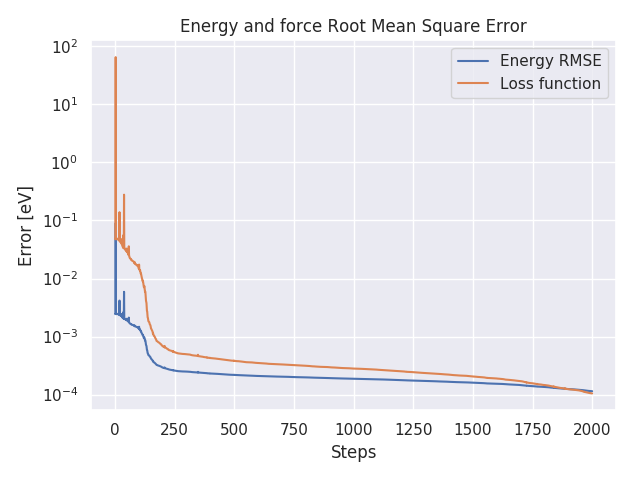
\includegraphics[width=\textwidth]{silicon_energy_log.png}
    \caption{Training loss and energy RMSE.}
  \end{subfigure}
  \hfill
  \begin{subfigure}[b]{0.55\textwidth}
      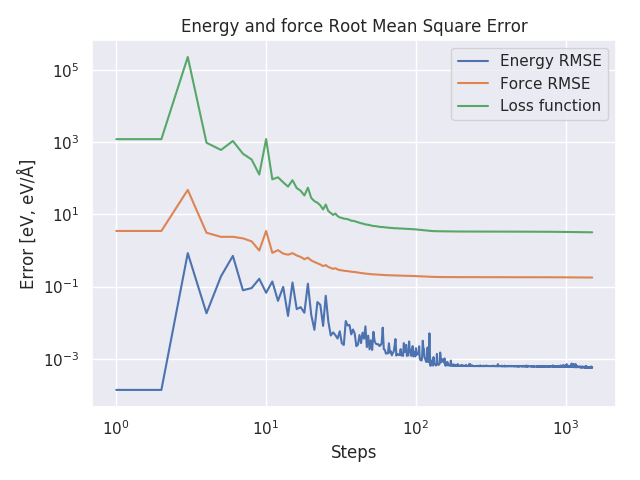
\includegraphics[width=\textwidth]{silicon_force_log.png}
    \caption{Training loss and energy and force RMSE.}
  \end{subfigure}
\end{adjustbox}
\caption{Training losses and energy and force root mean squared errors.}
    \label{fig:silicon-log}
\end{figure}

For both the energy training and the force training phases, the 
losses often rise sharply at the beginning, and then decay smoothly over time,
reaching something of a convergence after approximately 500-1000 steps.
The losses are somewhat higher for the Stillinger-Weber than for the
EMT potential, this may indicate more difficulty reproducing the distribution
or overfitting for the EMT potential.
This is also indicated in the test losses in figure \ref{fig:silicon-error},
where both the energy and force RMSEs are slightly higher than for the
EMT potential. This may also be an artifact of initialization, as finding
good high-dimensional minima using gradient descent is a process which in some cases
may require many restarts.
However, if we examine the energies interpolated over time,
it paints a better picture than for the EMT potential.
In figure \ref{fig:silicon-energy} we have plotted the energy as a function
of time. While the energy for the Stillinger-Weber potential is flat or oscillating
around a mean value over time, the neural network exhibits as before
a seemlingly linear increase in energy over time.
However, if we compare with the EMT potential the change over time is now significantly
smaller. This is also seen in the potential energy over time in figure \ref{fig:silicon-pot},
which is as before increasing, though the increase is smaller, and in general the potential
energy fits better than before.
We speculate on a few reasons for this, one is that since threebody terms are a significant
energy contribution to the potential energy the angular symmetry functions serve to
stabilize the system. 

\begin{figure}[H]
\begin{adjustbox}{max width=1.2\linewidth,center}
\centering
  \begin{subfigure}[b]{0.55\textwidth}
      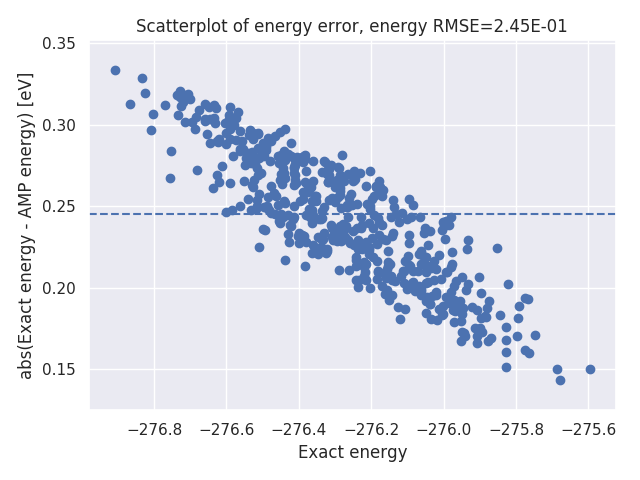
\includegraphics[width=\textwidth]{silicon_energy_error.png}
      \caption{Energy error.}
  \end{subfigure}
  \hfill
  \begin{subfigure}[b]{0.55\textwidth}
      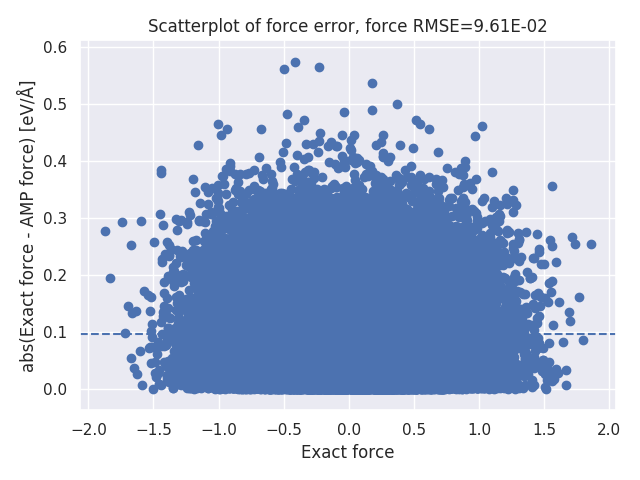
\includegraphics[width=\textwidth]{silicon_force_error.png}
      \caption{Force component error.}
  \end{subfigure}
\end{adjustbox}
    \caption{Energy and force component errors on test trajectory.}
    \label{fig:silicon-error}
\end{figure}

We expect in general that if the symmetry functions are not too correlated adding
more symmetry functions increase fit and numerical stability.
If we examine the radial distribution functions in figures
\ref{fig:copper-rdf} and \ref{fig:silicon-rdf} we find that the silicon system is more
highly peaked than the copper system, with fewer average number of neighbors.
This may also make this distribution easier to approximate for the silicon system
than for the copper system.

\begin{figure}[H]
    \centering
    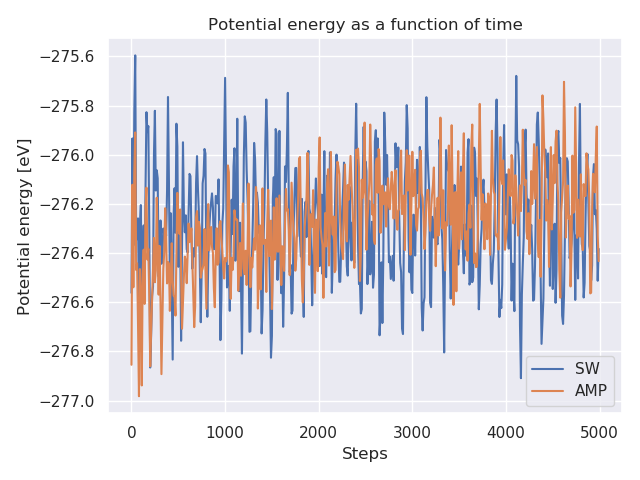
\includegraphics[width=\textwidth]{silicon_pot.png}
    \caption{AMP and Stllinger-Weber potential energy as a function of time.}
    \label{fig:silicon-pot}
\end{figure}

\begin{figure}[H]
    \centering
    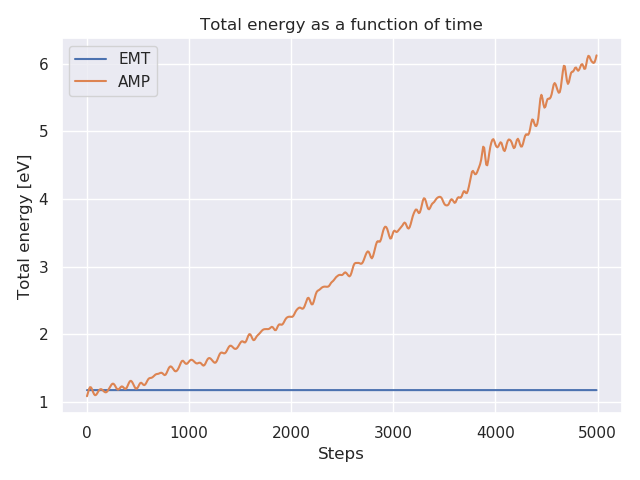
\includegraphics[width=\textwidth]{copper_energy.png}
    \caption{AMP and Stillinger-Weber total energy as a function of time.}
    \label{fig:silicon-energy}
\end{figure}

As before there are indications that the increase in energy is initially attributed
to the kinetic energy, as we see in the radial distribution functions the neural network
system is slightly more dispersed than the Stillinger-Weber system.
In addition in figure \ref{fig:silicon-msd} we can see that the mean squared
displacement is increasing in a non-linear fashion as the atoms pick up
both kinetic energy and translational momentum.

\begin{figure}[H]
    \centering
    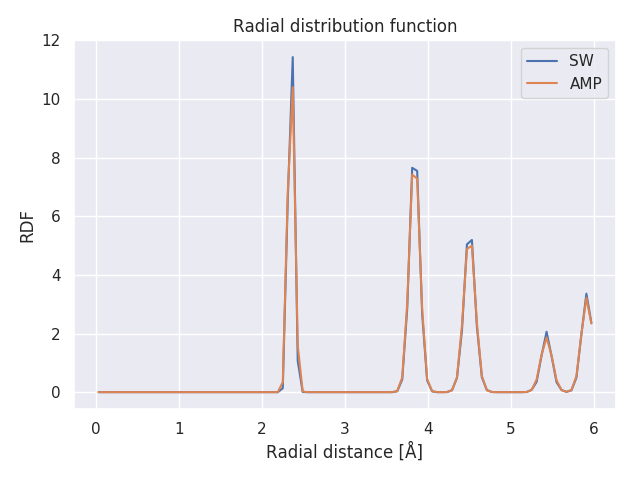
\includegraphics[width=\textwidth]{silicon_rdf.png}
    \caption{Radial distribution functions for the Stillinger-Weber and
        neural network potentials.}
    \label{fig:silicon-rdf}
\end{figure}

\begin{figure}[H]
    \centering
    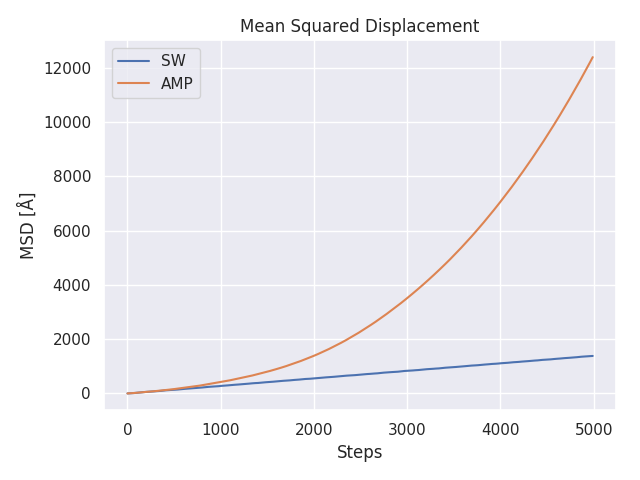
\includegraphics[width=\textwidth]{silicon_msd.png}
    \caption{Mean squared displacement over time for the Stillinger-Weber
        and neural network potentials.}
    \label{fig:silicon-msd}
\end{figure}

\begin{figure}[H]
\begin{adjustbox}{max width=1.2\linewidth,center}
\centering
  \begin{subfigure}[b]{0.55\textwidth}
      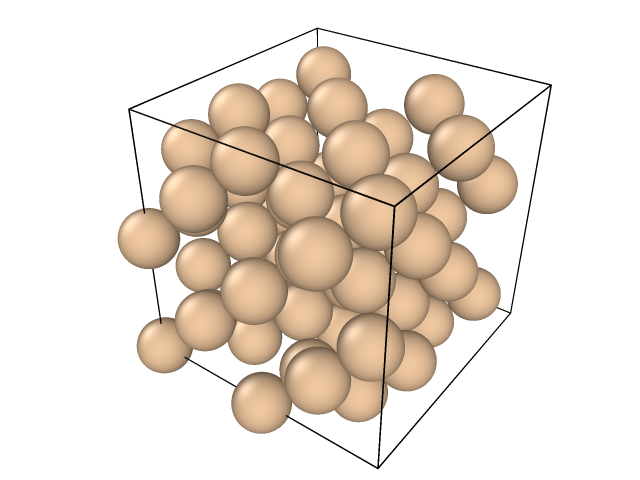
\includegraphics[width=\textwidth]{silicon_t0.png}
      \caption{Silicon atoms after 10 steps.}
  \end{subfigure}
  \hfill
  \begin{subfigure}[b]{0.55\textwidth}
      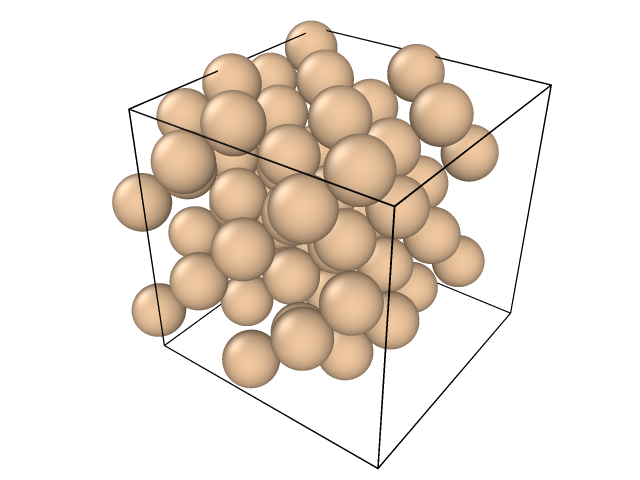
\includegraphics[width=\textwidth]{silicon_tn.png}
      \caption{Silicon atoms after 5000 steps.}
  \end{subfigure}
\end{adjustbox}
    \caption{The system of silicon atoms after 10 and 5000 steps.}
    \label{fig:silicon-time}
\end{figure}

The increase in kinetic energy and translational momentum is illustrated
both in the mean squared displacement and from snapshots of the system
as in figure \ref{fig:silicon-time}. This is even better illustrated
in visualization software, where we can see that while the
Stillinger-Weber system remains stationary over time, the neural network
system picks up momentum and starts moving.
We see that the system has moved slightly over time, while the crystal
structure has remained mostly intact as evidenced by the radial distribution
function.
However, since the energy conservation is better for the neural network
trained on the Stillinger-Weber potential, this motion is smaller
than what we have observed for the EMT potential.

\begin{figure}
    \centering
    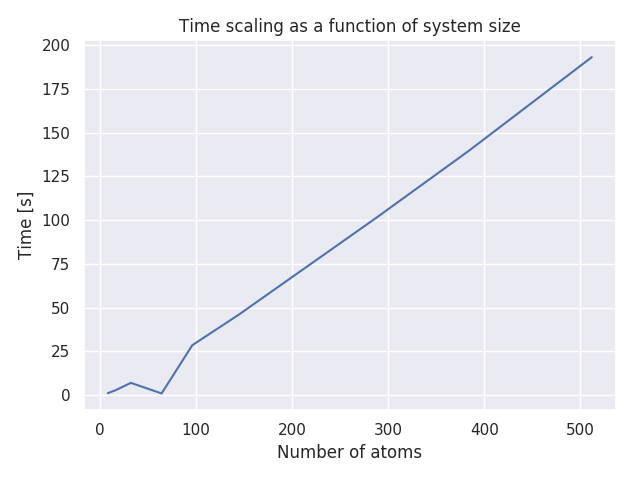
\includegraphics[width=\textwidth]{silicon_scaling.png}
    \caption{Time scaling of the neural network potential
        as a function of the size of the system.}
    \label{fig:silicon-scaling}
\end{figure}

Finally, we also examined the time scaling of the system as we did for the
neural network trained on the EMT potential.
As before we calculated the time it took for a single forces call
on all the atoms in the system, as this is the limiting
factor for integrating the atoms a single timestep using the
Verlet algorithm.
Ideally we would take averages of the time this takes, but except
for the smaller systems this does not affect the results very much,
due to the timescales involved.
The results are shown in figure \ref{fig:silicon-scaling}.
From this plot we observe that integrating a system
with 100 silicon atoms one step would take approximately
25-30 seconds, while a system of 300 atoms would take approximately
110 seconds. This means integrating a system of 100 atoms
for 5000 steps would take about 35 hours, which is quite
a large amount of time compared to typical empirical potentials.
For the Stillinger-Weber potential this force call
takes on the order of milliseconds, several orders of magnitude removed.
However, since the neural network potential scales linearly, this may be competive
with ab-initio methods which exhibit much poorer scaling as the system size increases.
Since we have added more radial and angular symmetry functions
we expect this to take much more time than for the copper system,
as angular derivatives are very expensive to evaluate for every atom.
Additionally, we used a slightly larger cutoff radius than for the copper system,
though the silicon system is less dense than the copper system, which also
affects the time to evaluate the atomic fingerprints and forces.
